\documentclass[a4, 11pt]{scrartcl}
%----------------------------------------
% German language
% \usepackage[ngerman]{babel}
%----------------------------------------
% Input in UTF8 accepted
%\usepackage[utf8]{inputenc}
%----------------------------------------
% Math-packages
\usepackage{mathtools}
\usepackage{amsmath}
\usepackage{amssymb}
%----------------------------------------
% Design choices (?)
%\usepackage{scrlayer-scrpage}
%\pagestyle{scrheadings}
% \clearscrheadfoot
%----------------------------------------
% Footnotes in tables
%\usepackage{tablefootnote}
%----------------------------------------
%----------------------------------------
% no parindent
\setlength{\parindent}{0em}
%----------------------------------------
% different gap between paragraphs
%\setlength{\parskip}{1.3ex}
%----------------------------------------
% spacing between lines
%\usepackage[onehalfspacing]{setspace}
%----------------------------------------
% Hurenkinder und Schusterjungen vermeiden
\clubpenalty = 10000
\widowpenalty = 10000
\displaywidowpenalty = 10000
%----------------------------------------
% Hyperref package
\usepackage{hyperref}
\hypersetup{
	colorlinks=true,
	linkcolor=black,
	filecolor=black,      
	urlcolor=OliveGreen,
	citecolor=black
}
%----------------------------------------
% Geometry package
\usepackage{geometry}
\geometry{
	paper=a4paper, % Change to letterpaper for US letter
	top=3cm, % Top margin
	bottom=3cm, % Bottom margin
	left=2cm, % Left margin
	right=3cm, % Right margin
	%showframe, % Uncomment to show how the type block is set on the page
}



\usepackage{float}

\usepackage{array, booktabs}
\usepackage{graphicx}
\graphicspath{ {./assets/} }
\usepackage[dvipsnames, table]{xcolor}
\usepackage{sectsty}
\sectionfont{\color{OliveGreen}}

\newcommand{\foo}{\color{OliveGreen}\makebox[0pt]{\textbullet}\hskip-0.5pt\vrule width 1pt\hspace{\labelsep}}

\usepackage{longtable}

\usepackage{wasysym}


\usepackage[framemethod=TikZ]{mdframed}

% Style %
\mdfdefinestyle{enviStyle}{
	innertopmargin = 10pt,
	linewidth      = 1pt,
	frametitlerule = true,
	roundcorner    = 2pt%
}


\newenvironment{CountingDefinition}[2][]{%
	\ifstrempty{#1}%
	{\mdfsetup{%
			frametitle={{\strut ~}}}
	}%
	{\mdfsetup{%
			frametitle={{\strut ~#1}}}%
	}%
	\mdfsetup{
		nobreak                   = true,
		linecolor                 = OliveGreen,
		frametitlebackgroundcolor = OliveGreen!50,
		style                     = enviStyle
	}
	\begin{mdframed}[]\relax%
		\label{#2}}{\end{mdframed}}



%\renewcommand{\labelitemi}{$\textcolor{OliveGreen}{\bullet}$}
\renewcommand{\labelitemii}{$\textcolor{Black}{\circ}$}
%\renewcommand{\labelitemiii}{$\textcolor{OliveGreen}{\diamond}$}
%\renewcommand{\labelitemiv}{$\textcolor{OliveGreen}{\ast}$}
\usepackage[htt]{hyphenat}

\newcommand{\heart}{\ensuremath\heartsuit}


%----------------------------------------
% References
%\usepackage[backend=biber, maxbibnames=99]{biblatex}
%\addbibresource{references.bib}
%----------------------------------------
%\ohead{\\
%		Pina Kolling\\
%		piko0011}
	
%\usepackage[vmargin=1in,hmargin=1in]{geometry}
%\usepackage{enumitem}
%\setlist[itemize]{topsep=0pt,before=\leavevmode\vspace{-1.5em}}
%\setlist[description]{style=nextline}

%----------------------------------------------------------------------------
%----------------------------------------------------------------------------

\begin{document}
	
	\title{\color{OliveGreen} \vspace{-5ex} Weekly Diary}
	\author{
		Master thesis course in Computing Science \\
		\textbf{Pina Kolling}
	}
	\date{\vspace{-5ex}}
	
	\maketitle
	 
	\begin{table}[H]
		\renewcommand\arraystretch{1.4}\arrayrulecolor{OliveGreen}
		\begin{longtable}{@{\,}r <{\hskip 2pt} !{\foo} >{\raggedright\arraybackslash}p{12cm}}
			% \toprule
			% \addlinespace[1.5ex]
			Week 3 & Introduction and first work on project plan \\
			Week 4 & Finish project plan, start setting up code on my computer  \\
			Week 5 & First research on the topic, including finding literature, set up Git and \LaTeX \ for master thesis (on work laptop, my laptop and stationary pc), document execution of code \\
			Week 6 & Set up code on my computer and first familiarizing with codebase, finding literature, document execution of code \\
			Week 7 & Researching options of melt framework (implementing, documenting the process and literature research)  \\
			Week 8 & Implementing, documenting the process and literature research and vacation with my grandmother (she turns 90 \heart) so probably reduced work capacity \\
			Week 9 & Implementing, documenting the process and literature research, evaluating if it is possible to obtain colour-corrected video results using JIT and then specify or readjust the focus \\
			Week 10 & Implementing, documenting the process and literature research and creating slides for the midterm seminar\\
			Week 11 & Implementing, documenting the process and literature research, midterm seminar \\
			Week 12 & Implementing, documenting the process and literature research, search or implement offline colour correction software and other suitable solutions for comparison (if needed) \\
			Week 13 &  Implementing, documenting the process and literature research \\
			Week 14 &  Implementing, documenting the process and literature research \\
			Week 15 &  Writing \\
			Week 16 &  Writing \\
			Week 17 &  Writing \\
			Week 18 &  Writing \\
			Week 19 &  Finalizing, reworking and applying feedback \\
			Week 20 &  Hand in final version of the thesis \\
			Week 21 &  Create Slides for the thesis seminar \\
			Week 22 &  Thesis seminar (defence and opposition) \\
			Week 23 &  Opponent thesis report \\
		\end{longtable}
	\end{table}


\newpage



	\section*{Week 3}
	
	\begin{description}
		








%-----------------------------------------------------------------------------		
		\item[16.01.24, Tuesday] 
		
		\begin{itemize}
			\item[]
			\item First meeting at university
		\end{itemize}








%-----------------------------------------------------------------------------		
		\item[17.01.24, Wednesday]
		
		\begin{itemize}
			\item[]
			\item Setting up file and git for weekly diary
			\item Writing first mail with topic specification to Vicen\c{c} Torra
			\item Keeping my supervisor at Codemill (Urban Söderberg) in the loop
			\item Begin with project plan (setting up the file, etc.)
		\end{itemize}








%-----------------------------------------------------------------------------		
		\item[18.01.24, Thursday]
		
		\begin{itemize}
			\item[]
			\item Getting a supervisor from university assigned (Cem Okulmus) % and first communication with him
			\item Continue work on project plan:
			\begin{itemize}
				\item Introduction
			\end{itemize}
			
			\item First research on:
			\begin{itemize}
				\item Just-In-Time (JIT), WebRTC, h.264, Melt framework
				\item Infrastructure model of the system
			\end{itemize}
		\end{itemize}







%-----------------------------------------------------------------------------		
\item[19.01.24, Friday]

\begin{itemize}
	\item[]
				\item Continue work on project plan:
	\begin{itemize}
		\item Problem formulation
		\item Method
		\item Infrastructure model
	\end{itemize}
\end{itemize}







%-----------------------------------------------------------------------------		
\item[20.01.24, Saturday]

\begin{itemize}
	\item[]
	\item Continue work on project plan:
	\begin{itemize}
		\item Evaluation methods
		\item Self assessment
	\end{itemize}
	\item Looking into previous master thesis that was written at Codemill
\end{itemize}

	\end{description}








%-----------------------------------------------------------------------------	
%-----------------------------------------------------------------------------	
\newpage
\section*{Week 4}

Info: The Codemill logo marks the days at which I have been at the company's office.

\begin{description}


%-----------------------------------------------------------------------------		
\item[22.01.24, Monday]
\begin{itemize}
	\item[]
	\item Set up git on other computer
		\item Continue work on project plan:
	\begin{itemize}
		\item Resources
		\item Read again and correct
		\item Deciding on a title
	\end{itemize}
	\item Send projectplan to supervisor at Codemill (Urban Söderberg)
	\item Send projectplan to supervisor at university (Cem Okulmus)
\end{itemize}







%-----------------------------------------------------------------------------		
\item[23.01.24, Tuesday]
\begin{itemize}
	\item[]
	\item First meeting with supervisor at university (Cem Okulmus)
	\item Rework and additional info on project plan:
	\begin{itemize}
		\item Change JIT definition
		\item Add timeline
		\item Add challenges
	\end{itemize}
	\item Add timeline weekly diary and adapt setup of weekly diary (counting in calendar weeks)
\end{itemize}








%-----------------------------------------------------------------------------		
\item[24.01.24, Wednesday]
\begin{itemize}
	\item[]
	\item Prepare laptop to set up code on it
\end{itemize}















%-----------------------------------------------------------------------------		
\item[25.01.24, Thursday]

\includegraphics[width=1.4cm]{codemill.png}
\begin{itemize}
	\item Setting up the code on my laptop at Codemill 
	
	(generating ssh key, cloning git repositories, installing node.js and docker, etc)
	\begin{itemize}
		\item Problem: My RAM was not sufficient and the code could not be executed
		\item Solution: Looking for a company laptop to execute the code
	\end{itemize}
\end{itemize}


















%-----------------------------------------------------------------------------		
\item[26.01.24, Friday]

\includegraphics[width=1.4cm]{codemill.png}
\begin{itemize}
	\item Setting up the code on the new laptop at Codemill
	\begin{itemize}
		\item Problem: Space in user name on the device which makes some paths not working
		\item Solution: Setting up windows with a new user (to do)
		\item Info: The code has not been run on a windows system before
	\end{itemize}
\end{itemize}

	\end{description}









%-----------------------------------------------------------------------------	
%-----------------------------------------------------------------------------	
\newpage
\section*{Week 5}

\begin{description}
	
	
%-----------------------------------------------------------------------------		
\item[29.01.24, Monday]
	\begin{itemize}
		\item[]
		\item Being sick \frownie{}
	\end{itemize}
	
	
	
	
	
	
	
%-----------------------------------------------------------------------------		
\item[30.01.24, Tuesday]
	\begin{itemize}
		\item[]
		\item Being sick \frownie{}
	\end{itemize}





%-----------------------------------------------------------------------------		
\item[31.01.24, Wednesday]
	\begin{itemize}
		\item[]
		\item Being sick \frownie{}
		\item Setting up new windows user
		\item Setting up code on new laptop (frontend running but problems with backend/docker container)
		\item Document execution of code:
	\end{itemize}




\end{description}
\vspace*{-0.8em}
\begin{CountingDefinition}[Setting up the code]{def:codesetup}
	\vspace*{-0.2em}
	\begin{itemize}
		\item Generate ssh key (\texttt{ssh-keygen}) and add to GitLab
		\item Clone git repositories (jit-webrtc and accurate-player-3-core)
		\item Install node.js and set path variables for npm (and yarn)
		\item Install and run docker
		\item Execute jit-webrtc code with command from README with \texttt{docker/main/main.sh --threads 16 --port 8080 \$VIDEOFILE} (not working!)
		\item Execute accurate player code (run \texttt{npm install --force}, \texttt{npm install yarn} and then npm start, resolve errors, fix dependenciy problems with \texttt{npm audit fix --force} (potentially twice))
	\end{itemize}
	
\end{CountingDefinition}

\begin{description}





%-----------------------------------------------------------------------------		
\item[01.02.24, Thursday]
\begin{itemize}
	\item[]
	\item Being sick \frownie{}
	\item Installing slack
	\item Looking into the backend/docker problem %(\texttt{docker: Error response from daemon: error gathering device information while adding custom device "C": not a device node.})
	\item Setting up WeeklyDiary git and tex file on Codemill-laptop
\end{itemize}






%-----------------------------------------------------------------------------		
\item[02.02.24, Friday]
\begin{itemize}
	\item[]
	\item Being sick \frownie{}
	\item Trying to solve the docker/backend problem (still unsolved)
	\item Setting up git and tex file for master thesis on stationary PC
	\item Creating title page
	\item Structure for thesis
	\item First research and adding of references
	\item First writing in introduction
\end{itemize}




%-----------------------------------------------------------------------------		
\item[03.02.24, Saturday]
\begin{itemize}
	\item[]
	\item Being sick \frownie{}
	\item Trying to solve the docker/backend problem (still unsolved):
	\begin{itemize}
		\item Inspecting \texttt{main.sh} script file
		\item Inspecting docker problems regarding windows
		\item \texttt{docker-run.sh} not found or opened... Changing the path does not seem to help and the file does exist (feedback: no such file or directory)
		\item Setting up python
	\end{itemize}
\end{itemize}


\end{description}








%-----------------------------------------------------------------------------	
%-----------------------------------------------------------------------------	
\newpage
\section*{Week 6}

\begin{description}

%-----------------------------------------------------------------------------		
\item[05.02.24, Monday]

\includegraphics[width=1.4cm]{codemill.png}
\begin{itemize}
	\item Run backend/docker (finally!): 
	\begin{itemize}
		\item Make changes in \texttt{main.sh} (last line): remove \texttt{--device /dev/fuse} and change path to  \texttt{//opt/jit-webrtc/jit/docker-run.sh}
	\end{itemize}
	\item Problem: Connectivity issues between browser and docker
	\item Solution: Installing Linux and not running it under Windows
\end{itemize}









%-----------------------------------------------------------------------------		
\item[06.02.24, Tuesday]
\begin{itemize}
	\item[]
	\item Installing Linux Ubuntu 22.04 (not booting after updates)
	\item Installing Linux Ubuntu 23.10 (does not work at all)
	\item Researching and writing an introduction about Codemill
	\item Installing Linux Ubuntu 22.04
	\begin{itemize}
		\item The problem originated from the NVIDIA graphics card. Before updating, the drivers had to be installed with \texttt{sudo ubuntu-drivers autoinstall}.
	\end{itemize}
	\item Installing docker, node.js, git, miktex, texstudio and cloning repositories
	\item Adding to weekly diary: Codemill logo for each day I was at the company's location
	\item Executing frontend
	\item Executing backend in docker container
\end{itemize}









%-----------------------------------------------------------------------------		
\item[07.02.24, Wednesday]

\includegraphics[width=1.4cm]{codemill.png}
\begin{itemize}
	\item Connecting backend and frontend
	\item Running the code
	\item Setting docker timeout from 15s to 150s in \texttt{main.py}
	\item Create private git repositories to store work progress 
	\item Research on WebRTC and transcoding and looking into code of JIT-WebRTC
	\item Adding labels and references to structure of master thesis tex file
	\item Adding README files of code base to master thesis tex file
\end{itemize}
\end{description}



\vspace*{-0.8em}
\begin{CountingDefinition}[Running the code] {def:coderun}
\vspace*{-0.2em}
\begin{itemize}
	\item Frontend: 
	\begin{itemize}
		\item Open folder \texttt{accurate-player-3-core/packages/demo} in terminal
		\item Execute \texttt{JIT\_BACKEND=http://localhost:8080 yarn start} or \texttt{./start.sh}
	\end{itemize}
	\item Backend:
	\begin{itemize}
		\item Open folder \texttt{jit-webrtc} in terminal
		\item Execute \texttt{docker/main/main.sh --threads 16 --port 8080 https://s3.eu-central-1.amazonaws.com/accurate-player-demo-assets/timecode/sintel-2048-timecode-stereo.mp4
		}
	\end{itemize}
	\item Open \url{http://localhost:5000/controls/jit/index.html} in browser
\end{itemize}

\end{CountingDefinition}

\begin{description}










%-----------------------------------------------------------------------------		
\item[08.02.24, Thursday]
% 
\includegraphics[width=1.4cm]{codemill.png}
\begin{itemize}
	\item[]
	\item Looking into the backend code, README and the system's components, summarizing and taking notes in the thesis file:
	\begin{itemize}
		\item Audio Video Interleave (AVI)
		\item Named pipe
		\item Create diagram of system
		\item Python documentation
		\item Web services and REST API
	\end{itemize}
	\item Structure of the thesis
\end{itemize}














%-----------------------------------------------------------------------------		
\item[09.02.24, Friday]
% 
\includegraphics[width=1.4cm]{codemill.png}
\begin{itemize}
	\item[]
	\item Looking into the backend code and the system's components, summarizing and taking notes in the thesis file:
	\begin{itemize}
		\item Docker container
	\end{itemize}
	\item Looking into the frontend code and README, summarizing and taking notes in the thesis file:
	\begin{itemize}
		\item Node.js, yarn and npm
	\end{itemize}
\end{itemize}



%-----------------------------------------------------------------------------			

		
		
\end{description}
	
	
	
	







%-----------------------------------------------------------------------------	
%-----------------------------------------------------------------------------	
\newpage
\section*{Week 7}	





\begin{description}
	
	
	
	
	
	%-----------------------------------------------------------------------------		
	\item[12.02.24, Monday]
	
\includegraphics[width=1.4cm]{codemill.png}
	\begin{itemize}
		\item Write to do list for the next steps and update time schedule
		\item Look into MLT FX and integration of OpenGL and GLSL?
		\item Looking into suitable filters (aka plugins) in melt
		\begin{itemize}
			
			\item Maybe suitable: \texttt{avfilter.colorbalance}, \texttt{avfilter.colorchannelmixer}, \newline \texttt{avfilter.colorcontrast}, \texttt{avfilter.colorlevels}, \newline \texttt{avfilter.colortemperature}, \texttt{frei0r.coloradj\_RGB}, \texttt{frei0r.colorize}
			
			
			\item Probably not suitable: \texttt{avfilter.colorcorrect}, \texttt{avfilter.colorhold}, \newline \texttt{avfilter.colorize}, \texttt{avfilter.colorkey}, \texttt{avfilter.colormatrix}, \newline \texttt{avfilter.colorspace}, \texttt{frei0r.colordistance}, \texttt{frei0r.colorhalftone}, \newline  \texttt{frei0r.colortap}, \texttt{frei0r.three\_point\_balance}, \texttt{frei0r.contrast0r}, \texttt{tcolor}
			
		\end{itemize}
	\end{itemize}
	

\end{description}	


% TODO
% ⚪️ literature research
% ⚪️ einleitung umstrukturieren und mehr auf farben beziehen
% ⚪️ look into code base
% ⚪️ mail an uni supervisor
% ⚪️ Abbildungs- und Tabellenverzeichnis
% Does melt already have an option for this?
	
	




\vspace*{-0.8em}
\begin{CountingDefinition}[To Do]{def:todo}
	\vspace*{-0.2em}
	
	\begin{itemize}
		\item Figure out, where the colour grading should be implemented
		\begin{enumerate}
			\item Does melt already have an option for this?
			\item Can it maybe only be done when the video is paused?
			\item Is there a different place in the system, where the colour grading can be done?
		\end{enumerate}
	\end{itemize}
	
\end{CountingDefinition}







\begin{description}
	
	
	\item[13.02.24, Tuesday]
	
\includegraphics[width=1.4cm]{codemill.png}
	\begin{itemize}
		\item Looking briefly into \texttt{melt.c}, \texttt{JitControl.proto}, \texttt{JitStatus.proto} and other melt files to find out, where to attach a filter/plugin to a video and where the quality setting is changed
		% \item Looking briefly into proto 3 syntax
		\item Getting first overview over structure of melt
		\item Execute melt with filter without JIT to test the filters: \texttt{melt https://s3.eu-central-1.amazonaws.com/accurate-player-demo-assets/timecode/sintel-2048-timecode-stereo.mp4 -filter avfilter.colorbalance av.rs=1 av.gm=1 av.bh=1} for intense colours
	\end{itemize}


\begin{minipage}{0.5\textwidth}
	
\includegraphics[width=0.9\textwidth]{colourdefault.png}
	Original colours
\end{minipage}\begin{minipage}{0.5\textwidth}
	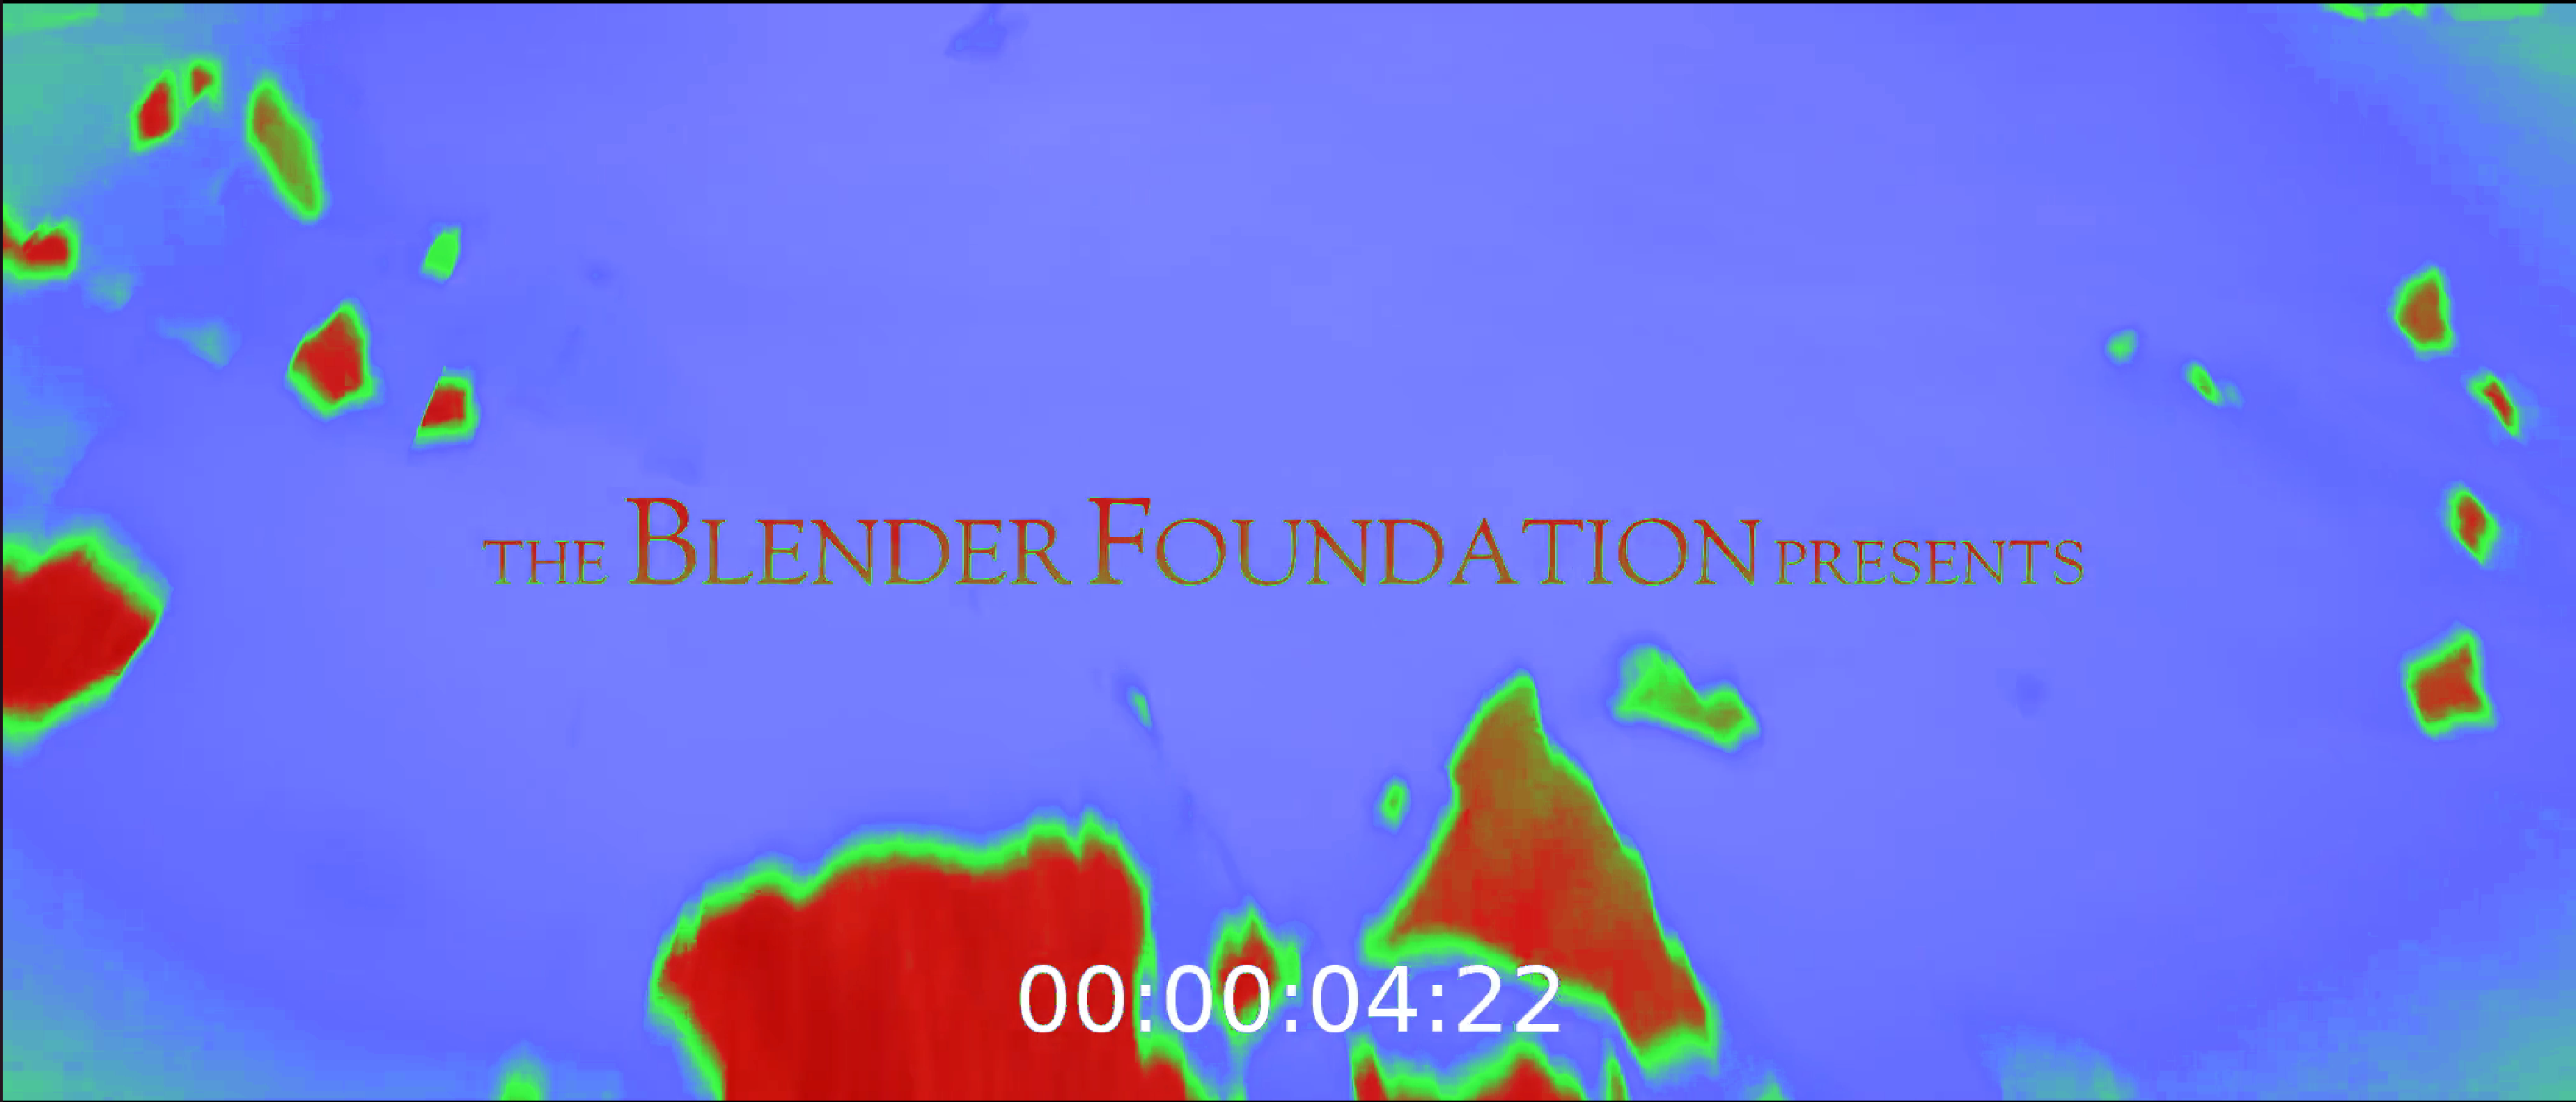
\includegraphics[width=0.9\textwidth]{colourhigh.png}
	Colours with \texttt{av.rs=1} \texttt{av.gm=1} \texttt{av.bh=1}
\end{minipage}

\begin{itemize}
	\item[$\rightarrow$] This can be used for the offline comparison
	\item Starting to look into \texttt{local\_melt.py}
\end{itemize}

	
	
\end{description}	


	
	
	
	
\end{document}